\documentclass{report}
\usepackage{ctex}
\usepackage{geometry}
\usepackage{graphicx}
\usepackage{subfigure}
\usepackage{amsmath}
\title{人工智能第一次实验实验报告}
\author{舒文炫}
\date{\today}
\geometry{a4paper,left=2cm,right=2cm,top=1cm,bottom=1cm}
\begin{document}
    \maketitle
    \tableofcontents
    \chapter{实验介绍}
    \section{实验内容}
    本次实验分两个部分,分别是Search和multiagent
    \begin{itemize}
        \item Search目标是吃豆人寻找食物,即静态查找算法,本次实验需要实现
        BFS算法和A*算法。
        \item Multiagent的目标是吃完所有食物同时避开鬼,其目的是在有对手的情况下
        做下一步决策使得自己利益最大化,这里需要实现minimax算法和alpah-beta剪枝。
    \end{itemize}
    \section{实验环境}
    Python3.6,我使用了anaconda来管理python环境,脚本运行使用了Git Bash。
    \chapter{实验设计}
    \section{part1:search}
    要完成BFS算法,需要有一个数据结构,可以保存当前节点的所有子节点,且子节点的访问顺序要在所有上一层节点
    访问完成之后,这样使用队列就很合适,队列可以实现数据先进先出,父节点先进,子节点在所有父节点后面。从前往后依次访问即可\par 
    对A*算法,需要一个启发式函数(这个助教已经给出,只要调用即可)以及当前路径总代价,加起来算做总代价的估计,
    我们每次选择代价最小的扩展,这样可以考虑使用优先队列,代价越小,优先级越高,就在队列越前面,这样依次扩展优先队列节点即可。\par 
    比较方便的是,助教已经给出了队列以及优先队列这些数据结构,可以直接使用。
    \section{part2:multiagent}
    对minimax算法,我们需要在博弈树上搜索,所提供的参数有搜索的深度,即往后看的回合数,以及ghost的数量,对每个状态,需要判断
    该状态是agent操作还是ghost操作,对agent节点我们要选最大的那个,对ghost节点我们要选最小的那个。由于这个博弈树,状态信息都已经封装好了,我在这里
    完成的为节点的选择。由于深度不一定为1,我考虑的框架是调用minimax函数递归,遍历当前节点所有的子节点,对深度为1,可以直接返回结果,大于1的可以通过深度为1
    的子问题间接得到。对深度为1的情况,由于ghost的数目不一定为1,即取min结点的次数不会仅为1次,此时都是在同一深度,这里就需要判断在当前状态应该取max还是min。
    观察发现:agent节点需要取max,ghost节点要取min,但是要注意一点,ghost后可能还会接ghost,当ghost后面是agent时,是当次博弈结束,如果深度为1可以直接返回结果,
    如果深度大于1,此时深度要减1。\par 
    对alpha-beta剪枝算法,这是对minimax的改进,剪枝使得我们没必要扩展所有的节点,我们可以将一些情况剪去,从而加快搜索。
    主体仍选择minimax算法所描述的方式,需要加上alpha,beta参数,保存到目前为止路径上发现的MAX极大值以及MIN极小值。
    在max节点处若发现拓展的点的值比beta值大,则后面的情况直接剪去,即返回到上层递归的位置。在min节点处若发现拓展的点的值比alpha值小,则后面的情况直接剪去,即返回到上层递归的位置。\par 
    \chapter{算法实现}
    下面我将展示我的代码来解释具体实现:
    \section{part1:search}
    \begin{figure}[h]
        \centering
        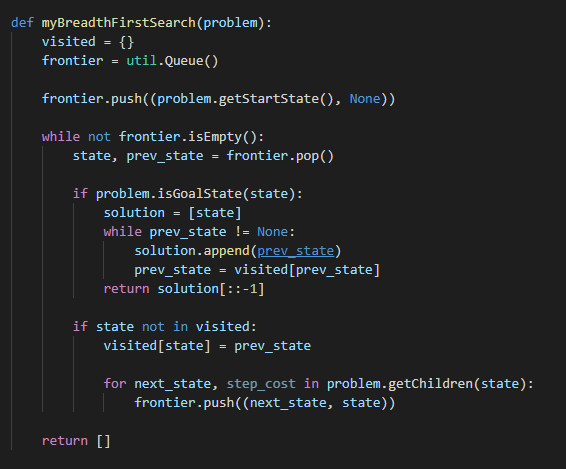
\includegraphics[width=15cm]{1.png}
        \caption{BFS}
    \end{figure}
    初始化frontier为queue(队列),先将开始节点入队列,进入循环,只要frontier队列不空,将其第一个元素出队列,判断其是否为终止态,是则结束,此时找到了一条路径。
    若不是,更新visited字典,表示该节点已经扩展过,键是当前状态,值是其父节点,从而visited字典可以用来保存一条到达终点的路径。再循环将其所有子节点入队列,这个就实现了广度优先。
    \begin{figure}[h]
        \centering
        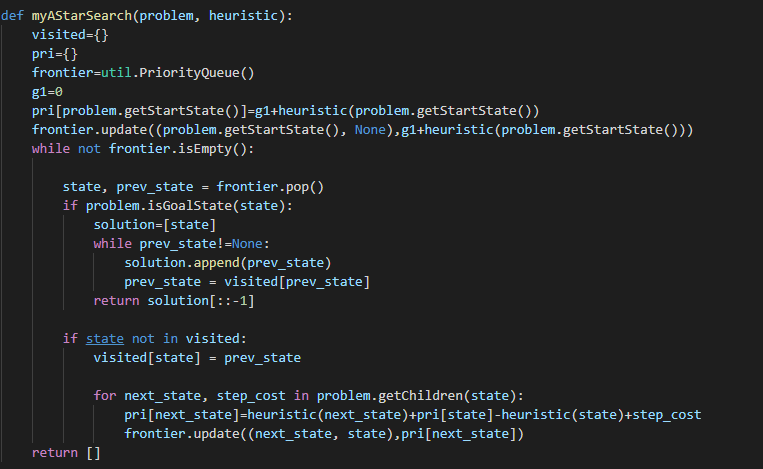
\includegraphics[width=15cm]{2.png}
        \caption{A* search}
    \end{figure}
    这里的框架与BFS基本相同,我们用到了priorityqueue这个数据结构,维护它用到的是堆排序算法。计算优先级的方法,由于不能直接得到到当前节点路径的代价,只有每一步的代价,我保存了一个pri数组,用来储存
    每个节点n的pri值,即$$pri(n)=h(n)+g(n)$$。h(n)的值我们可以直接调用heuristic函数得到。那么下一个节点next的优先值$$pri(next)=pri(n)-h(n)+step\_cost+h(next)$$
    然后使用update函数去更新队列,将最小值放在队列的头,方便之后pop出去。
    \section{part2:multiagent}
    \begin{figure}[h]
        \centering
        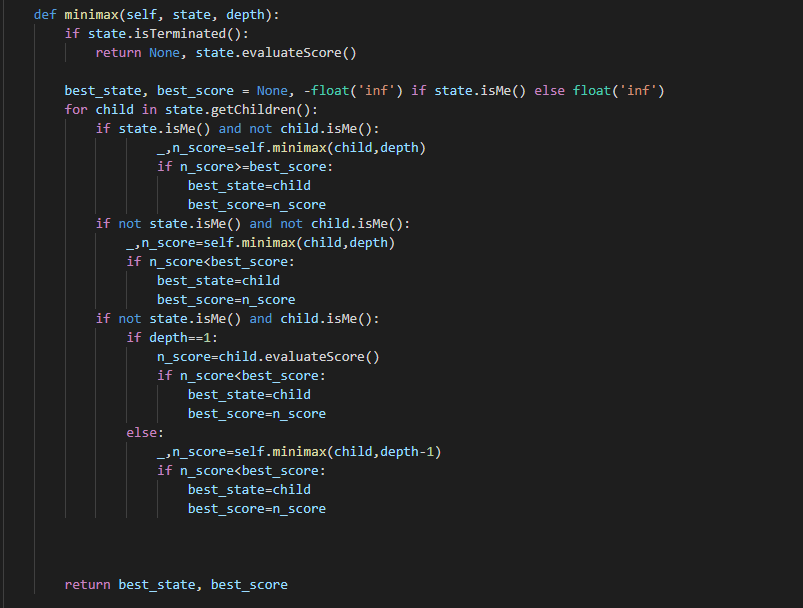
\includegraphics[width=15cm]{3.png}
        \caption{minimax}
    \end{figure}
    minimax函数用来递归,如果当前状态是终止状态则直接返回该状态的值,若不是,进入到下面主体,按照我在实验设计里面的描述,我将情况分为了三种
    \begin{itemize}
        \item 当前状态为agent下一个为ghost,此时对所有子节点找max,同时递归深度不变。
        \item 当前状态为ghost下一个为ghost,此时对所有子节点找min,同时递归深度不变。
        \item 当前状态为ghost下一个为agent,此时对所有子节点找min,递归深度减1,此时进入到了下一回合,深度为1时需要直接返回,作为递归的出口。
    \end{itemize}
    最后返回最佳状态和最好的值。\par 
    \begin{figure}[ht]
        \centering
        \subfigure[alpha-beta cut part1]{
            \begin{minipage}[t]{0.5\linewidth}
                \centering
                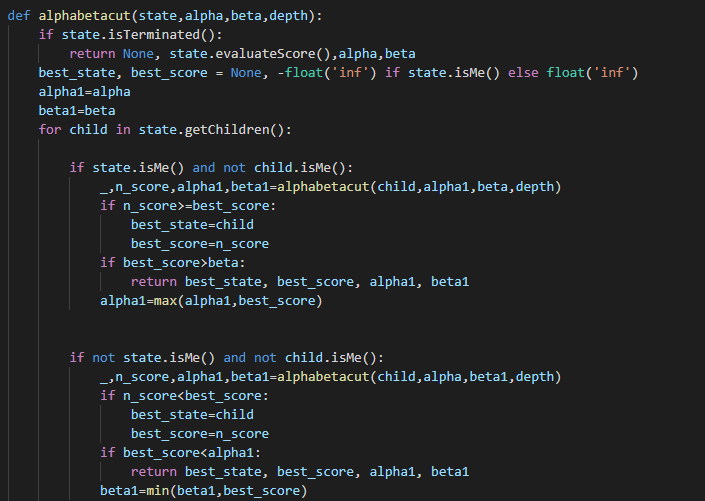
\includegraphics[width=12cm]{4.png}

            \end{minipage}
        }
        \subfigure[alpha-beta cut part2]{
            \begin{minipage}[t]{0.5\linewidth}
                \centering
                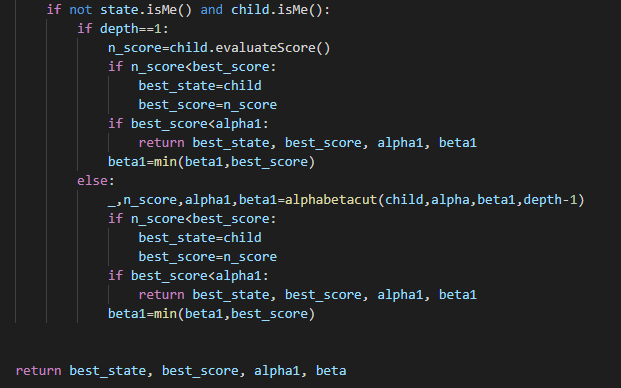
\includegraphics[width=12cm]{5.png}

            \end{minipage}
        }
    \end{figure}
    alpha-betacut算法和minimax主体相同,这里我直接在getNextState函数里面定义了alphabetacut函数方便进行递归。这里多出了两个参数alpha,beta,其含义在
    实验设计里面已经提过。我这里仅指出与minimax函数不同的地方。中间变量alpha1,beta1用来保存临时的alpha,beta值
    \begin{itemize}
        \item 当前状态为agent下一个为ghost,此时对所有子节点找max,同时递归深度不变,这时在原来的层,可能会修改alpha值,所以需要传入alpha1,即改变后的alpha值。若发现拓展的点的值比beta值大,则后面的情况直接剪去,即返回到上层递归的位置。
        \item 当前状态为ghost下一个为ghost,此时对所有子节点找min,同时递归深度不变,这时在原来的层,可能会修改beta值,所以需要传入beta1,即改变后的beta值。若发现拓展的点的值比alpha值小,则后面的情况直接剪去,即返回到上层递归的位置。
        \item 当前状态为ghost下一个为agent,此时对所有子节点找min,递归深度减1,此时进入到了下一回合,深度为1时需要直接返回,作为递归的出口。传参与上一条相同。
    \end{itemize}
    getNextState函数主体:设置alpha,beta初始值以及调用了alphabetacut函数。
    \begin{figure}[h]
        \centering
        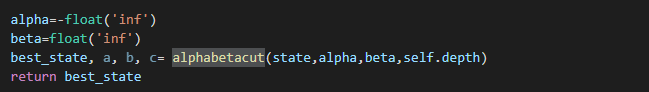
\includegraphics[width=15cm]{6.png}
        \caption{getnextstate}
    \end{figure}
    \chapter{实验测试以及结果分析}
    \section{part1: search}
    测试结果以图形化界面表示:
    \begin{figure}[h]
        \centering
        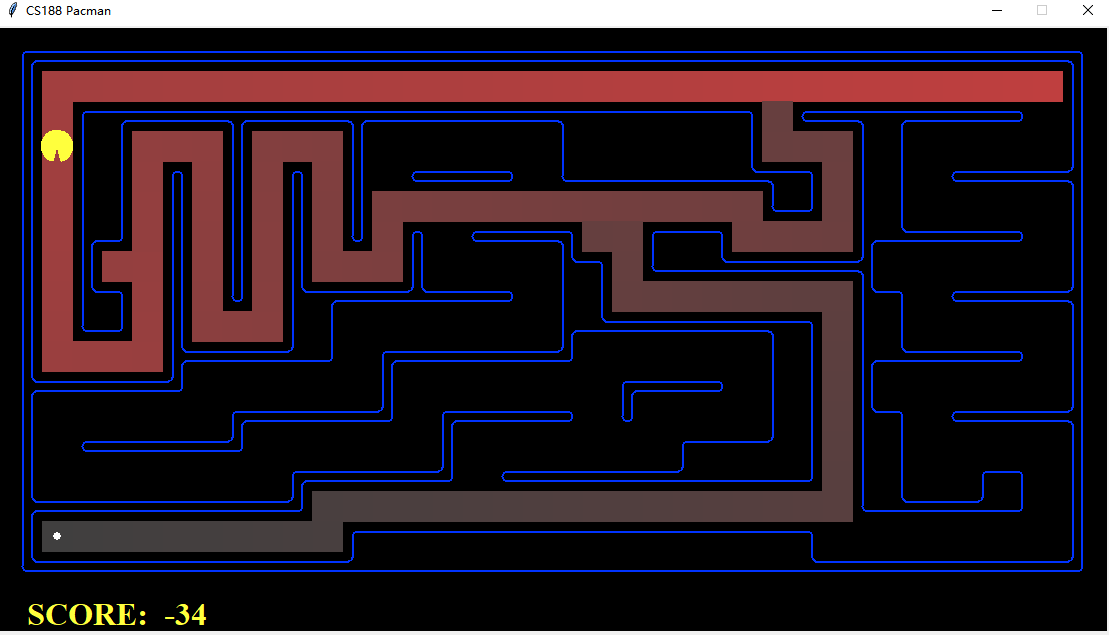
\includegraphics[width=15cm]{7.png}
        \caption{DFS}
    \end{figure}
    \begin{figure}[h]
        \centering
        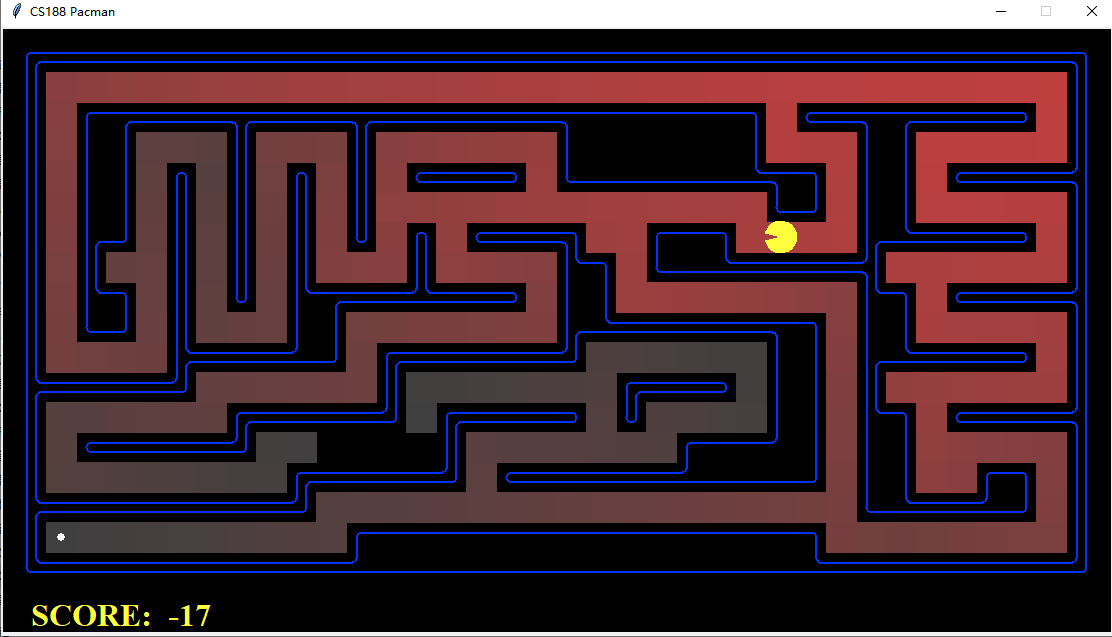
\includegraphics[width=15cm]{8.png}
        \caption{BFS}
    \end{figure}
    \begin{figure}[h]
        \centering
        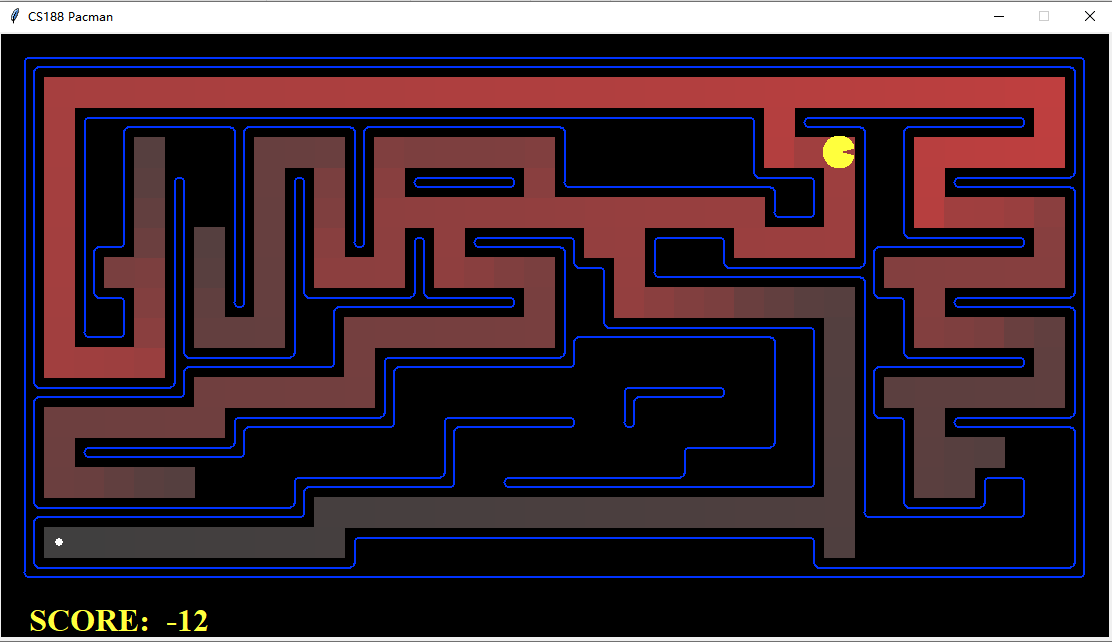
\includegraphics[width=15cm]{9.png}
        \caption{A*}
    \end{figure}
这三幅图,分别对应三种算法搜索扩展的节点,红色表示扩展的路径节点,比较三幅图,我们发现DFS算法,扩展的节点是最少的,这是因为该算法会对一条路径走到底,
如果发现了目标就结束,这里扩展的路径比较好,很快找到了目标。BFS算法扩展的节点是最多的,这是它每下一层,都会把该层所有节点遍历一遍,然而在大多数情况下,
这些扩展是没有意义的。这两个算法是无信息搜索,A*算法是有信息搜索,我们知道了启发式函数以及每一步的代价,扩展的节点少一些,这里扩展出了一条代价最小的路径。

\section{part2:multiagent}
这里测试的时候,对所有测试样例都PASS,说明我的算法实现正确。
\chapter{实验总结}
本次实验,我实现了DFS,A*,minimax,alphabetacut四个算法,进一步了加深了对算法的理解,以及算法实现能力,收获很大。
\end{document}

